\documentclass[xcolor=x11names]{beamer}
\usefonttheme{serif}
\usepackage{amsmath, amssymb, color, graphicx}
\usepackage{subcaption}
\usepackage{graphicx}

\def\bi{\begin{itemize}}
\def\ei{\end{itemize}}
\def\bn{\begin{enumerate}}
\def\en{\end{enumerate}}
\def\i{\item}

\newcommand{\argmax}{\operatorname*{arg \ max}}


\title{Applications of topological data analysis to single-cell genomics}
\author{Keshav Motwani}
\date{\today}


\begin{document}


\frame{\titlepage}

\frame{
	\frametitle{Background}
	\bi
		\i Single-cell RNA sequencing (scRNA-seq) allows us to measure gene expression in thousands of cells at once
		\i Previously, only bulk RNA-seq was possible, meaning the observed gene expression was the result of summing across all cells within a sample
		\i scRNA-seq is scientifically useful as it allows us to understand what role specific cell types play in biological processes
		\i Resulting data is in the form of a cells by genes matrix (approximately 30,000 genes) per sample
	\ei
}

\frame{
	\frametitle{Application}
	
		\bi
			\i Is it possible to detect differences in gene expression caused by treating blood cells with Interferon-$\gamma$?
			\bi
				\i Interferon-$\gamma$ is known to induce a variety of immune responses.
			\ei
			\i What cell types does Interferon-$\gamma$ modulate?
			\vspace{0.7cm}
			\i Dataset:
				\bi
					\i Kang et al. 2018 published scRNA-seq data from blood cells pre- and post-treatment for a total of 8 patients
					\i Every cell is annotated with a cell type label 
				\ei
		\ei
}

\frame{
	\frametitle{Motivation for using TDA}
		\bi
			\i We want to understand differences in the distribution of cells in gene expression space that is caused by a treatment, which fits perfectly into the TDA workflow described in class for point clouds
			\i Currently, there exist no published methods to classify entire scRNA-seq samples other than to simply average gene expression over all cells in the sample, and applying standard classification algorithms on the averaged data
			\bi
				\i No benefit over older bulk RNA-seq technology with that method
			\ei
		\ei
}

\frame{
	\frametitle{Data preprocessing}
		\bi
			\i Filter out dead cells and doublets
			\i Represent each sample based on it's top 50 principal components
				\bi
					\i For computational feasibility in computing pairwise Euclidian distances
				\ei
		\ei
}

\frame{
	\frametitle{Data example (one patient, pre-treatment)}
	\centering
	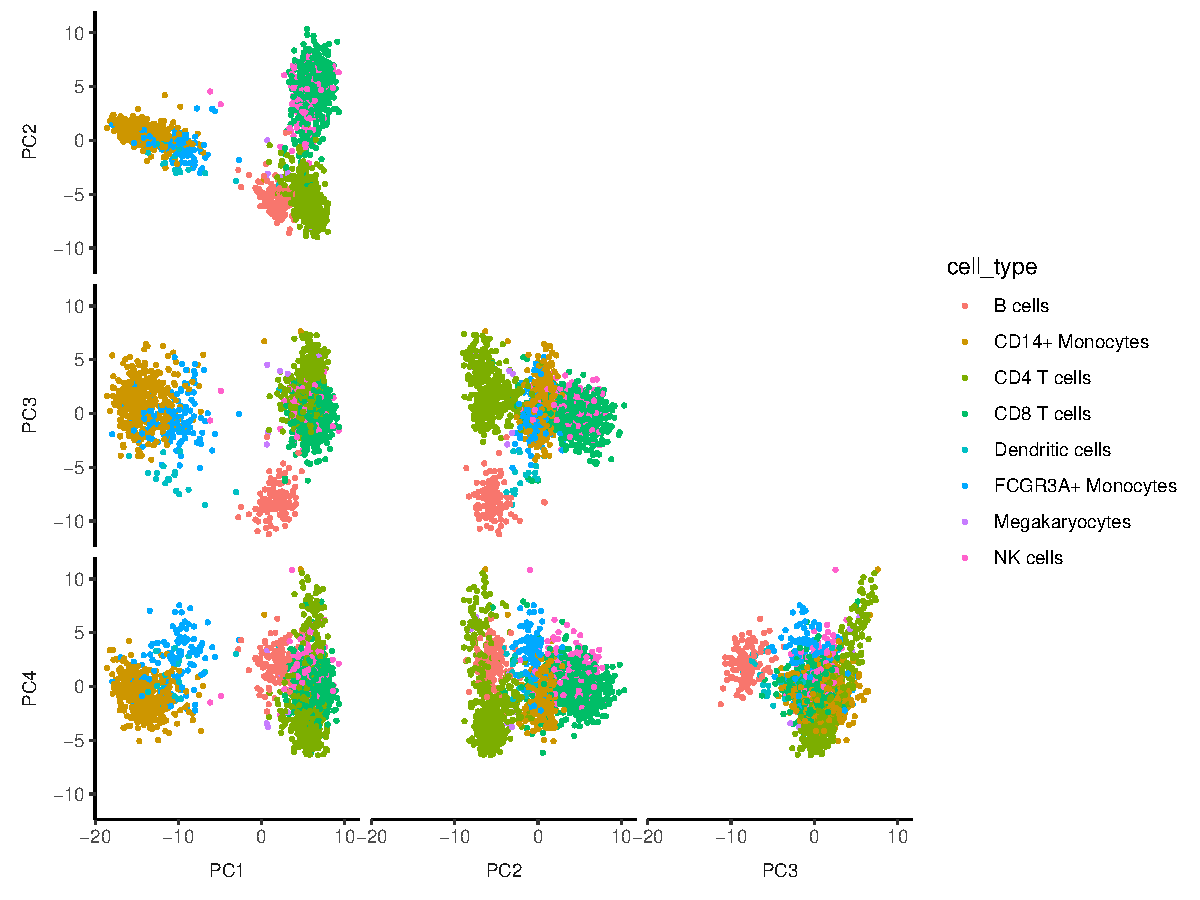
\includegraphics[width=10cm]{results/example_data.pdf}
}

\frame{
	\frametitle{Simplicial complex construction}
		\bi
			\i Vietoris-Rips complex with varying radius
			\i 200 values of radius equally spaced from $0$ to $R$, where $R$ is chosen to be the $0.1$ quantile of the values inside the pairwise distance matrices
		\ei
}

\frame{
	\frametitle{Persistent homology computations}
	Let A be one scRNA-seq sample. We consider $p \in \lbrace 0, 1 \rbrace$.
		\bi
			\i We have
$$
{\rm VR}_1(A) \subset {\rm VR}_2(A)	 \subset \cdots \subset {\rm VR}_{200}(A).
$$
			\i Compute homology in degree $p$
$$
H_p({\rm VR}_j(A)) = Z_p({\rm VR}_j(A))/B_p({\rm VR}_j(A))
$$ 
			\i We get
$$
H_p({\rm VR}_1(A)) \mapsto H_p({\rm VR}_2(A)) \mapsto \cdots \mapsto H_p({\rm VR}_{200}(A)).
$$
			\i Then we compute barcodes and persistence landscapes for statistics and machine learning
		\ei
}

\frame{
	\frametitle{Features in $H_0$ and $H_1$}
	\centering
	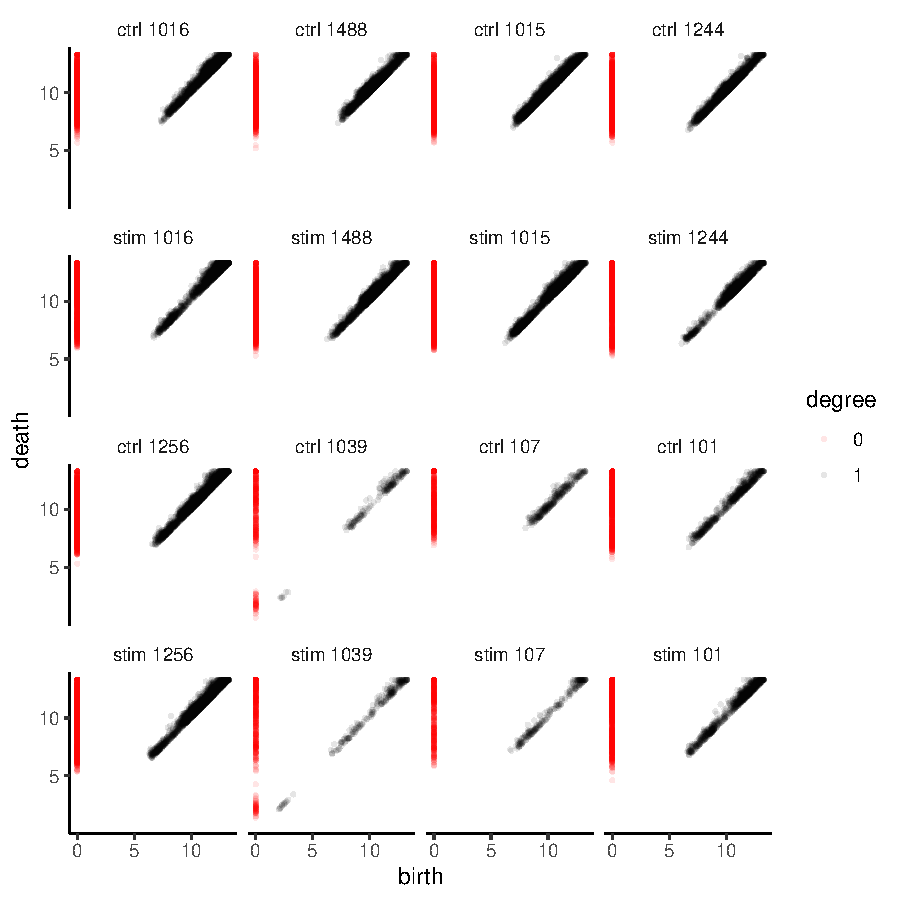
\includegraphics[width=8cm]{results/all_persistence_diagrams.pdf}
}

\frame{
	\frametitle{$H_1$ barcodes}
	\centering
	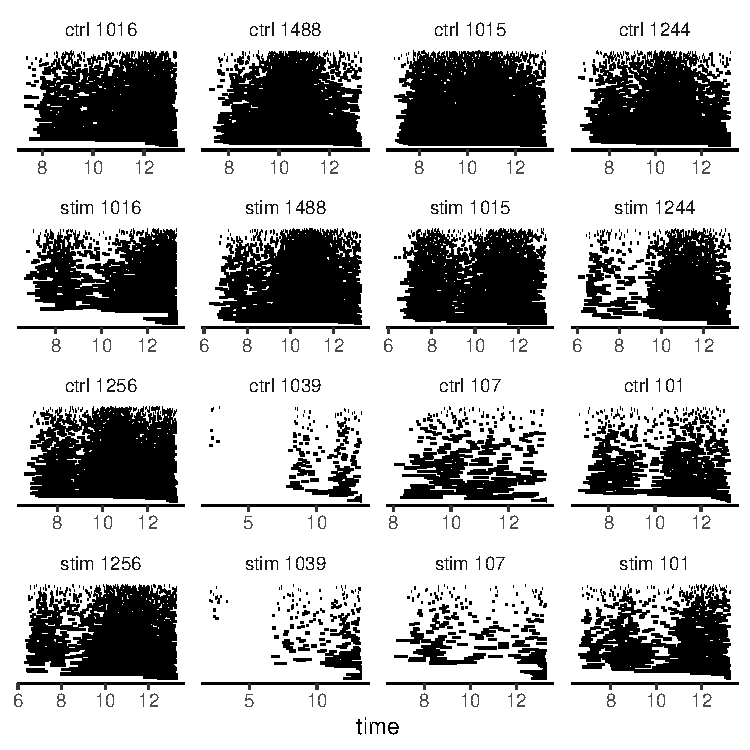
\includegraphics[width=8cm]{results/all_barcodes.pdf}
}

\frame{
	\frametitle{Persistence landscapes}
	\centering
	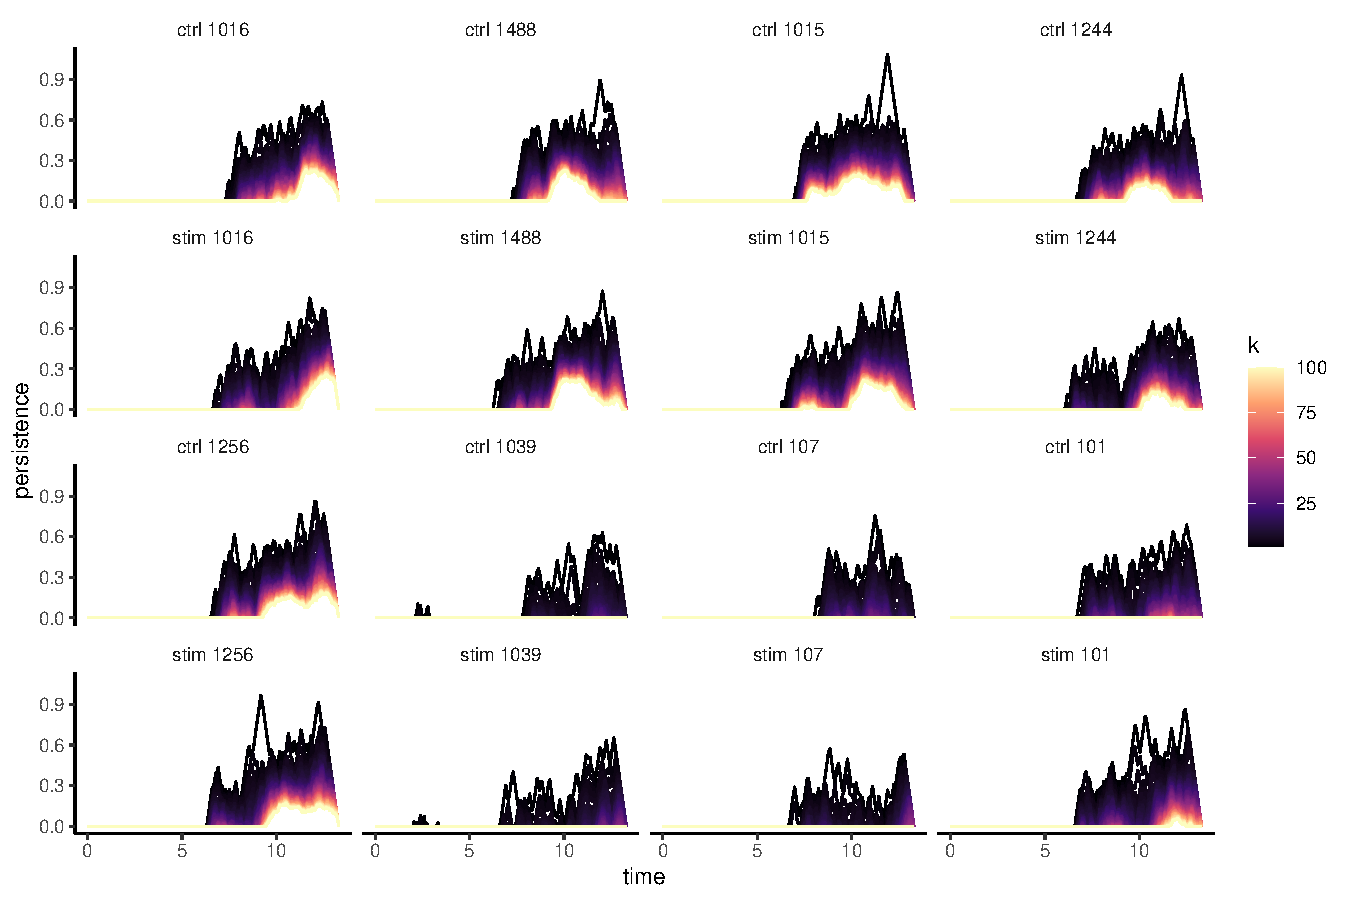
\includegraphics[width=10cm]{results/all_persistence_landscapes.pdf}
}

\frame{
	\frametitle{Average persistence landscape difference}
		Some features that: 
				\bi
					\i persist longer in earlier timepoints post-treatment
					\i persist longer in middle timepoints pre-treatment
					\i persist longer in later timepoints post-treatment
				\ei
	\centering
	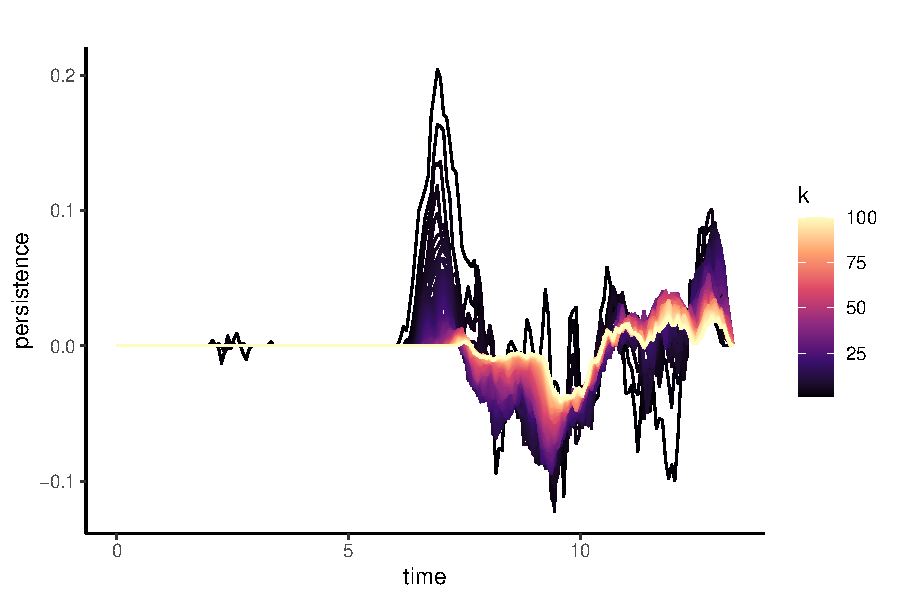
\includegraphics[width=8cm]{results/all_persistence_landscape_difference.pdf}
	
}

\frame{
	\frametitle{PCA on persistence landscapes}
	There is separation by treatment status in PC2, generally post-treatment has lower PC2 values
	\begin{center}
		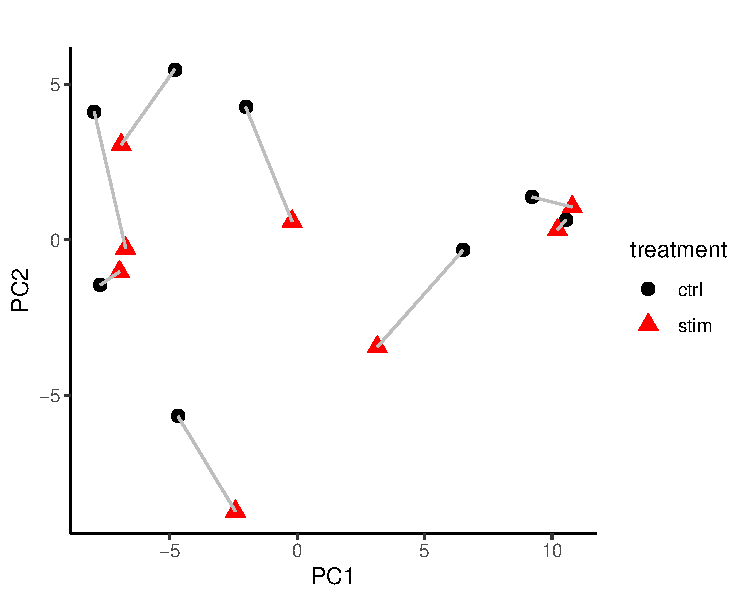
\includegraphics[width=8cm]{results/all_persistence_landscape_pca.pdf}
	\end{center}
}

\frame{
	\frametitle{Paired sample permutation test}
	Let $X_i \sim F({\rm PL}(X_i))$ and $Y_i \sim F({\rm PL}(Y_i))$ denote the pre- and post-treatment sample from the $i$th patient respectively, and ${\rm PL}(\cdot)$ be the true persistence landscape vector. 
		\bi
			\i Want to test the null hypothesis that ${\rm PL}(X_i) = {\rm PL}(Y_i)$
		\ei
	Test statistic: 
		\bi 
			\i $T(X, Y) = ||\frac{1}{N}\sum_{i = 1}^{N} \hat{{\rm PL}}(X_i) -  \hat{{\rm PL}}(Y_i) ||_2$
			\i Same as two-sample test statistic
		\ei
	Null distribution:
		\bi
			\i Construct permutations that permute treatment status only within the same patient, let $X^*, Y^*$ denote the permutations where
$$
X^*_i = X_i~\text{or}~Y_i, \quad
Y^*_i =   \begin{cases}
               	X_i & \text{if $X^*_i = Y_i$} \\
                  Y_i & \text{otherwise} \\
 			 \end{cases}
$$
			\i There are $2^N$ such permutations
		\ei
}

\frame{
	\frametitle{Permutation test}
	\centering
	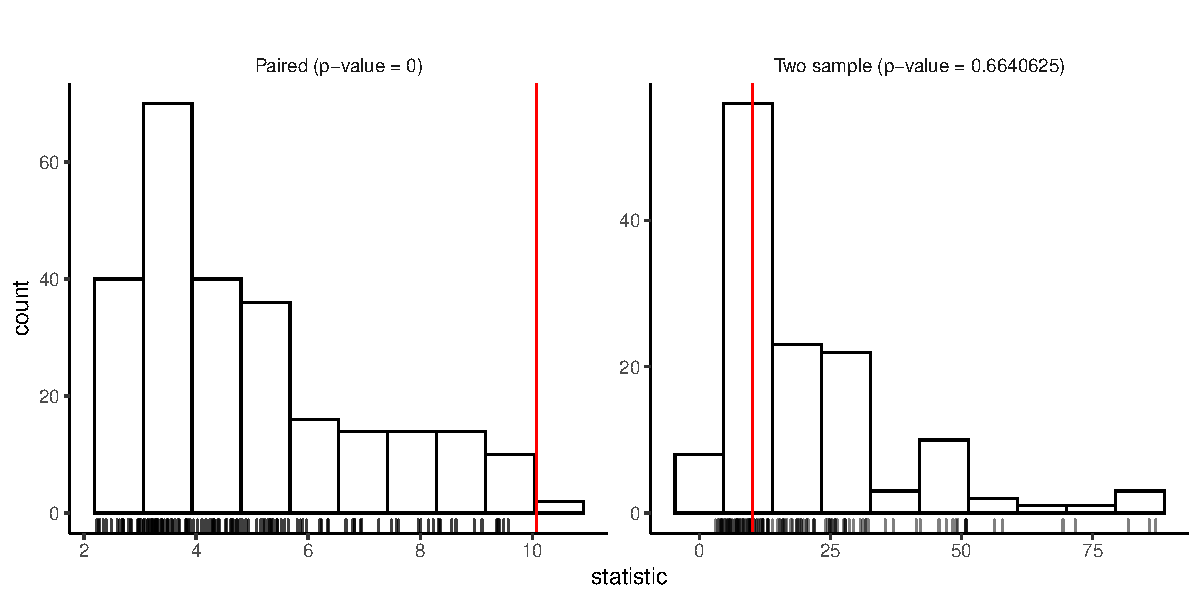
\includegraphics[width=10cm]{results/all_permutation_test.pdf}
}

\frame{
	\frametitle{Average persistence landscape difference per cell type}
	\centering
	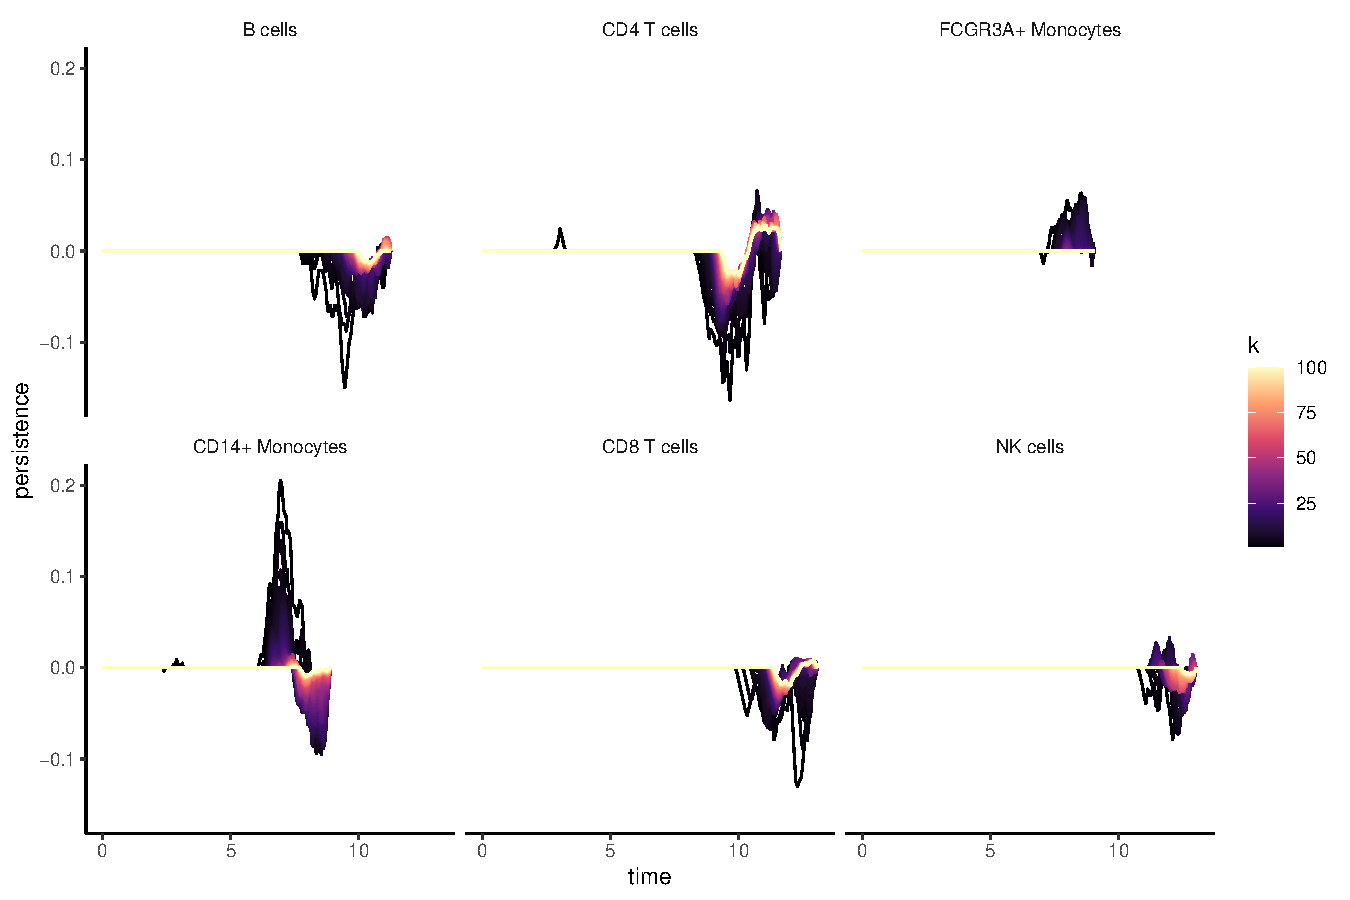
\includegraphics[width=10cm]{results/combined_persistence_landscape_difference.pdf}
}

\frame{
	\frametitle{PCA on persistence landscapes per cell type}
	\centering
	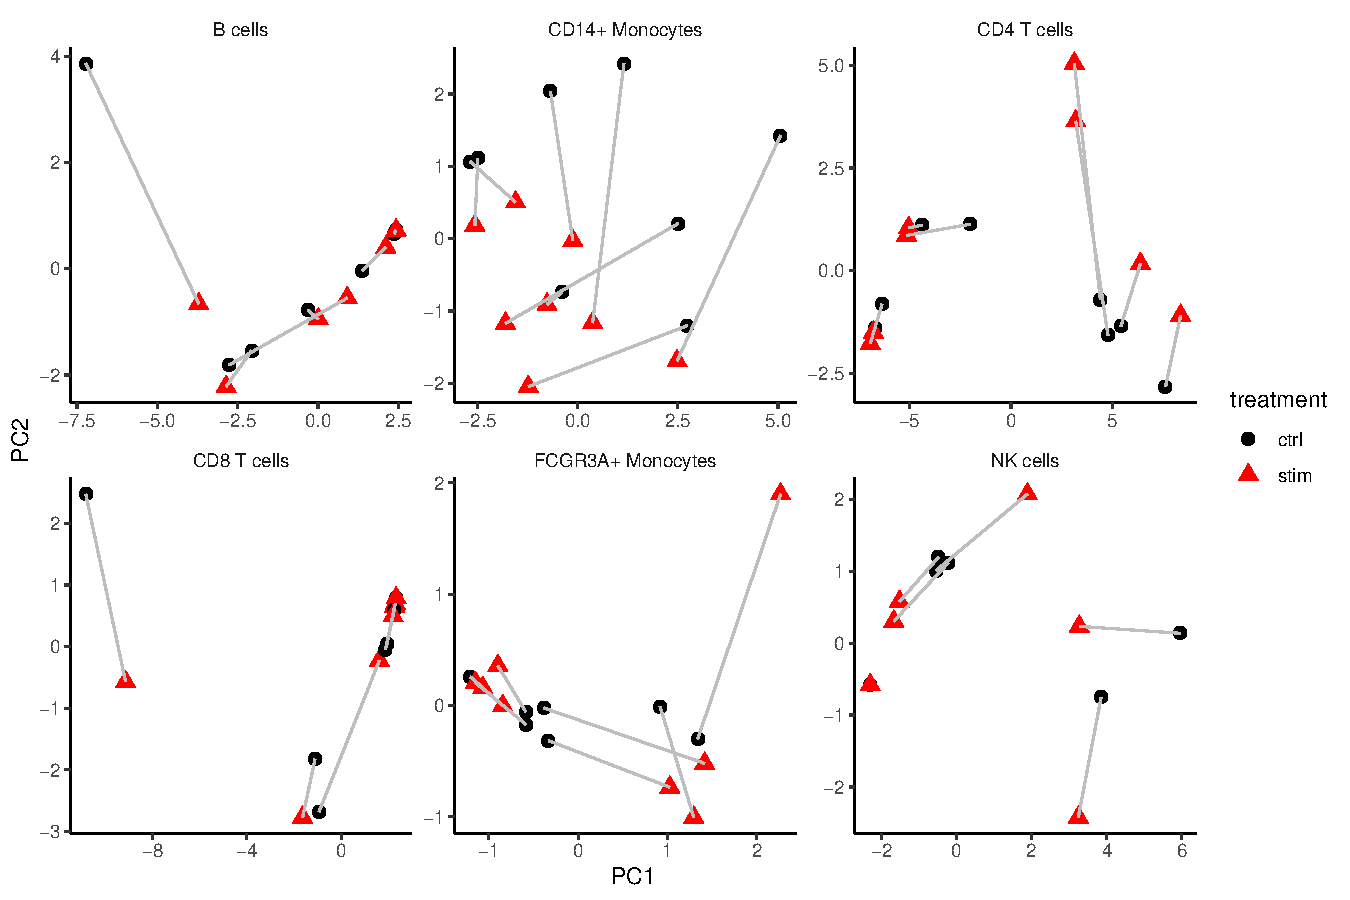
\includegraphics[width=10cm]{results/combined_persistence_landscape_pca.pdf}
}

\frame{
	\frametitle{Permutation test per cell type}
	\centering
	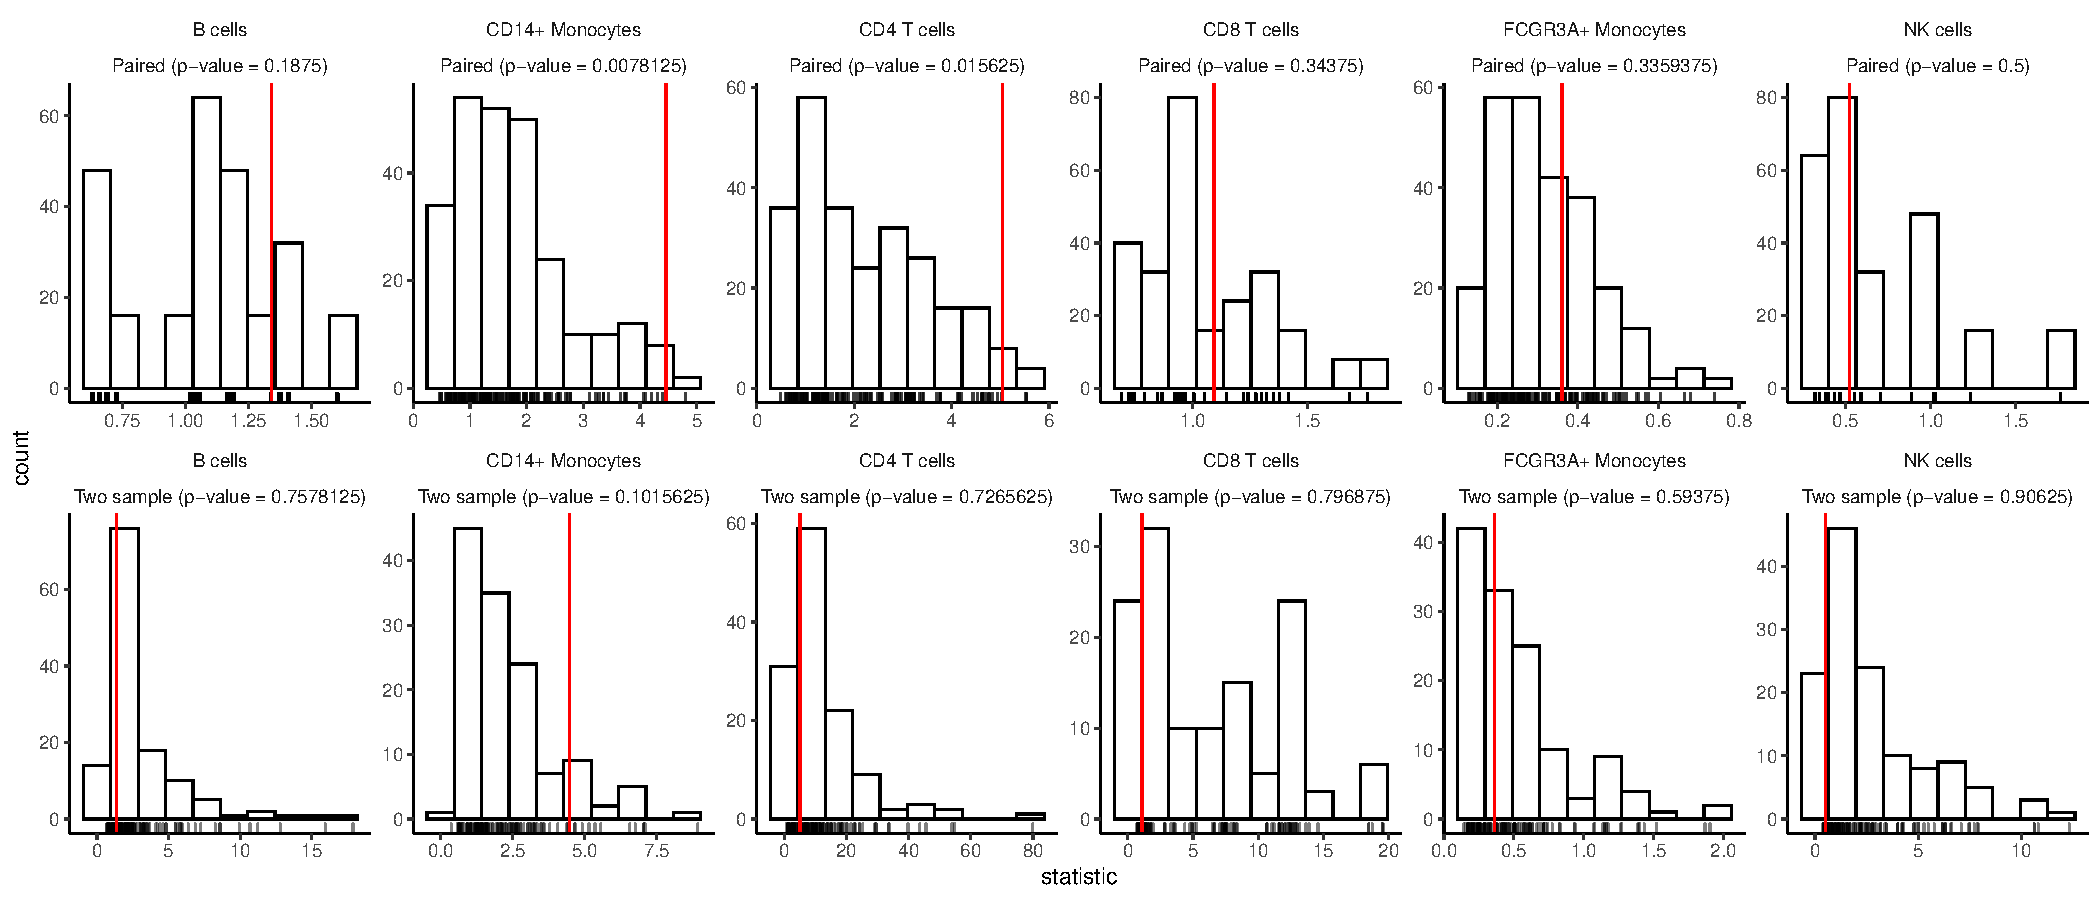
\includegraphics[width=11cm]{results/combined_permutation_test.pdf}
}

\frame{
	\frametitle{Conclusions}
		\bi
			\i Persistence landscapes show differences pre- and post-treatment in the same patient
			\i CD14+ Monocytes and CD4+ T cells show the largest differences after Interferon-$\gamma$ treatment
			\i Topological data analysis is a promising method for single-cell genomics and should be explored further
		\ei
}

\end{document}